\begin{enumerate}[label=\thesection.\arabic*.,ref=\thesection.\theenumi]
\numberwithin{equation}{enumi}

\item
In the Feedback System given below 
\begin{align}
\label{eq:ee18btech11035_G(s)}
 G(s)=\frac{1}{s^2+2s}
\end{align}
The step response of the closed-loop system should have minimum settling time and have no overshoot\\

\begin{figure}[!ht]
    \begin{center}
		
		\resizebox{\columnwidth}{!}{\tikzset{
        block/.style = {draw, rectangle,
            minimum height=1cm,
            minimum width=2cm},
        input/.style = {coordinate,node distance=1cm},
        output/.style = {coordinate,node distance=4cm},
        arrow/.style={draw, -latex,node distance=2cm},
        pinstyle/.style = {pin edge={latex-, black,node distance=2cm}},
        sum/.style = {draw, circle, node distance=1cm},
}

\begin{tikzpicture}[node distance=2.5cm,auto,>=latex']
  \node [input, name=input] {};
  \node [sum, right of=input] (sum) {};
  \node [block, right of = sum] (block1) {$k$};
  \node [block, right of = block1] (block2) {$G(s)$};
  \node [output, right of= block2] (output) {};
  \draw [->] (input) -- node {$r$} (sum);
  \draw [->] (sum) -- node {} (block1);
  \draw [->] (block1) -- node {} (block2);
  \draw [->] (block2) -- node [name =y] {$y$} (output);
  \draw [->] (y) -- ++ (0,-2) -| node [pos=0.99] {$-$} (sum);
\end{tikzpicture}}
	\end{center}
\caption{Block Diagram of given question}
\label{fig:block2}
\end{figure}

\item The required value of gain 'k' to achieve this is\\
\solution \\$Settling time$ : The time required for the transient's damped oscillations to
reach and stay within ±2\% of the steady-state value.\\
\\$Overshoot$ : The amount that the waveform overshoots the steady state, or final, value at the peak time, expressed as a percentage of the steady-state
value.\\

The Transfer function of the negative unity feedback system is given by 

\begin{align}
H(s)=\frac{G(s)}{1+G(s)H(s)}
\label{eq:1}
\end{align}
Where G(s) is the open loop gain of the feedback system and H(s) is the gain of feedback system \\
In our case
 \begin{align}
G(s) = k*G(s) = kG(s)
\label{eq:2}\\
H(s) = 1
\label{eq:3}
\end{align}
\\
From \eqref{eq:1} , \eqref{eq:2} and \eqref{eq:3}\\
Transfer function of Whole feedback system becomes

 \begin{align}
H(s) = \frac{kG(s)}{1+kG(s)}
\label{eq:4}
\end{align}

From \eqref{eq:ee18btech11035_G(s)} Substituting G(s) in \eqref{eq:4} \\
\\Our Transfer Function becomes 
\begin{align}
H(s) = \frac{k*\frac{1}{s^2+2s}}{1+k*\frac{1}{s^2+2s}}
\end{align}
On further simplifying we get,\\
\begin{align}
H(s) = \frac{k}{s^2+2s+k}
\label{eq:H(s)}
\end{align}\\
\\
Depending upon the value of 'k' the system can be : \\
\begin{itemize}
    
\item Undamped System
\item Underdamped System
\item Critical Damped System
\item Over Damped System 

\end{itemize}
\\
\\Plot of various types of systems in time domain:
\\
\begin{figure}[!h]
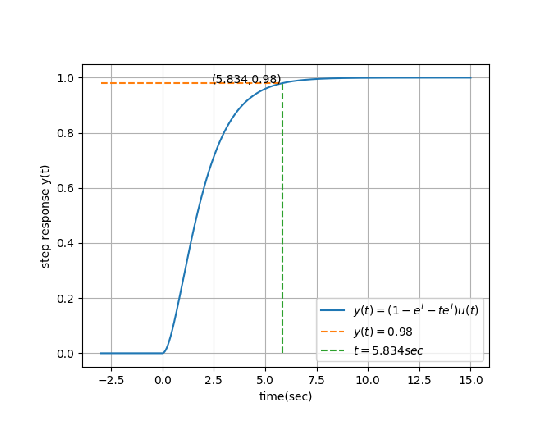
\includegraphics[width=\columnwidth]{./figures/ee18btech11035_1.eps}
\caption{Different Types of systems}
\label{fig:ee18btech11035_different_systems}
\end{figure}\\
Python code for the above plot is
\begin{lstlisting}
codes/ee18btech11035_1.py
\end{lstlisting}

\\Now, graphically observing the system which has minimum settling time and also doesn't overshoot.\\
\\From Figure:\eqref{fig:ee18btech11035_different_systems}
\\The system with minimum settling is critical damped system also this system doesn't overshoot.
\\
\\
So,when unit step is given as an input for critical damped system the output of the system has minimum settling time also the output doesn't overshoot.\\
\\
So, our transfer function H(s) should be a critical damped system.\\
The general form of a second order system is 

\begin{align}
H(s) = \frac{\omega_n^2}{s^2+2\zeta\omega_ns+\omega_n^2}
\label{eq:general_transfer_function}
\end{align}
where \(\zeta \)  is the damping factor \\
\begin{itemize}
\item \(\zeta \) = 0 for a undamped system
\item \(0 < \zeta  < 1\) for a underdamped system
\item \(\zeta  = 1\) for a critical damped system
\item \(\zeta  > 1\) for a overdamped system
\end{itemize}
\\
\\
In our case the damping factor for H(s) is 1 as it should be critical damped system \\

By comparing the equations \eqref{eq:H(s)} and \eqref{eq:general_transfer_function}
We get,

\begin{align}
\omega_n^2 = k\\
\label{eq:omega}
\omega_n = \sqrt{k}\\
2\zeta\omega_ns = 2s\\
\label{eq:zetaomega}
\zeta\omega_n = 1
\end{align}

From \eqref{eq:omega} and \eqref{eq:zetaomega} \\
\begin{align}
\zeta\sqrt{k} = 1
\label{eq:zetarootk}
\end{align}
As \(\zeta\) = 1 \eqref{eq:zetarootk} becomes 
\begin{align}
\sqrt{k} = 1\\
k = 1
\end{align}

Therefore, Transfer function is 
\begin{align}
H(s) = \frac{1}{s^2+2s+1}
\end{align}

\item 
Plot of Transfer function.
\\ \solution  
\begin{figure}[!h]
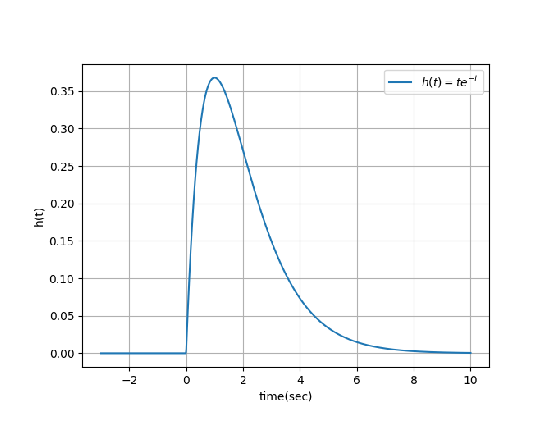
\includegraphics[width=\columnwidth]{./figures/ee18btech11035_2.eps}
\caption{Plot of h(t)}
\label{fig:ee18btech11035_h(t)}
\end{figure}

Python code for the above plot h(t) is
\begin{lstlisting}
codes/ee18btech11035_2.py
\end{lstlisting}

\begin{align}
H(s) = \frac{1}{s^2+2s+1}\\
\implies H(s) = \frac{1}{(s+1)^2}
\end{align}

Calculating the time domain equivalent for the transfer function\\
\begin{align}
\label{eq:s}
\frac{1}{s} = u(t)\\
\label{eq:s+1}
\frac{1}{s+1} = e^{-t}u(t)\\
\label{eq:(s+1)^2}
\frac{1}{(s+1)^2} = te^{-t}u(t)\\
\end{align}
Therefore,
\begin{align}
h(t) = te^{-t}u(t)
\end{align}


\item 
Plot of Output when input is unit step.

\\ \solution
\begin{figure}[!h]
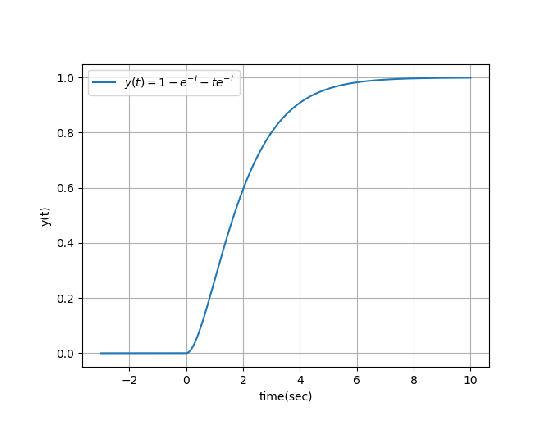
\includegraphics[width=\columnwidth]{./figures/ee18btech11035_3.eps}
\caption{Plot of y(t)}
\label{fig:ee18btech11035_y(t)}
\end{figure}

Python code for the above plot y(t) is
\begin{lstlisting}
codes/ee18btech11035_3.py
\end{lstlisting}


\\
We know that
\begin{align}
x(t) = u(t)
\end{align}
Converting x(t) in s-domain 
\begin{align}
X(s) = \frac{1}{s}\\
Y(s) = H(s)*X(s)\\
Y(s) = \frac{1}{(s+1)^2}*\frac{1}{s}
\end{align}
Converting Y(s) into partial fraction\\
We get,
\begin{align}
Y(s) = \frac{1}{s}-\frac{1}{s+1}-\frac{1}{(s+1)^2}
\end{align}
Converting Y(s) into y(t)\\
As mentioned in \eqref{eq:s}, \eqref{eq:s+1} and \eqref{eq:(s+1)^2}\\
\begin{align}
y(t) = (1-e^{-t}-te^{-t})u(t)
\end{align}


\end{enumerate}
